\begin{frame}[label=p26_20260920]{7v17: fine Punzi scan selects xeff 30\%}
\begin{columns}[T]
\column{0.49\textwidth}\centering\textbf{Versus score}\par
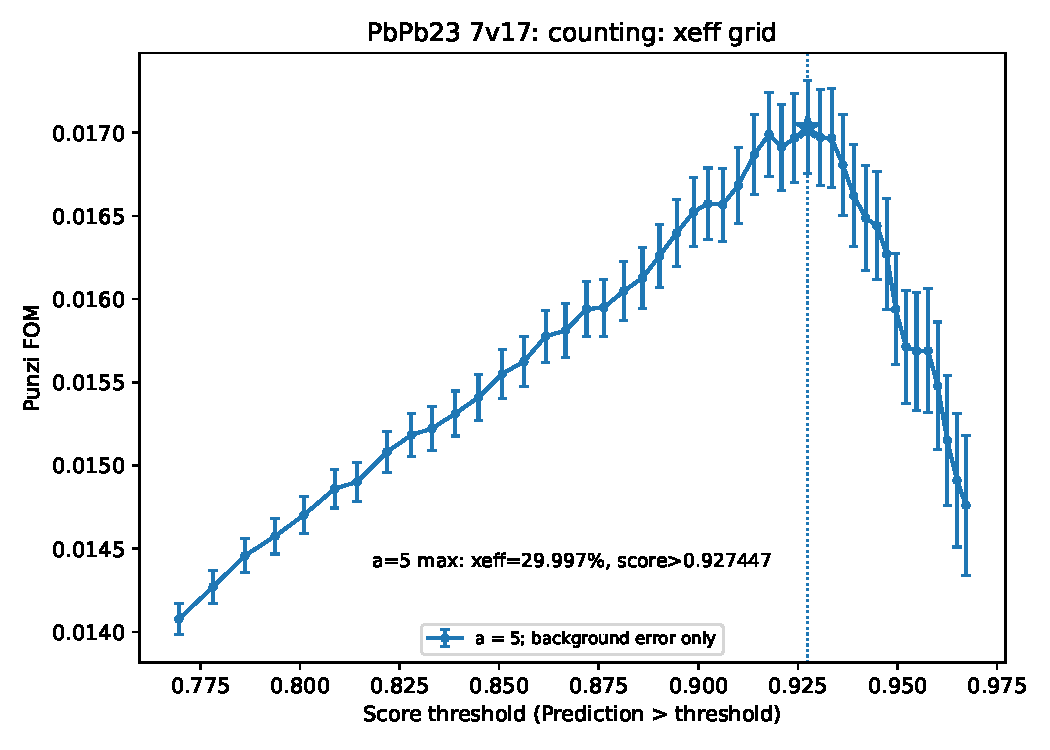
\includegraphics[width=\linewidth,height=0.56\textheight,keepaspectratio]{figures/20260920/punzi/7v17_xeff_scan_vs_score.pdf}
\column{0.49\textwidth}\centering\textbf{Versus xeff}\par
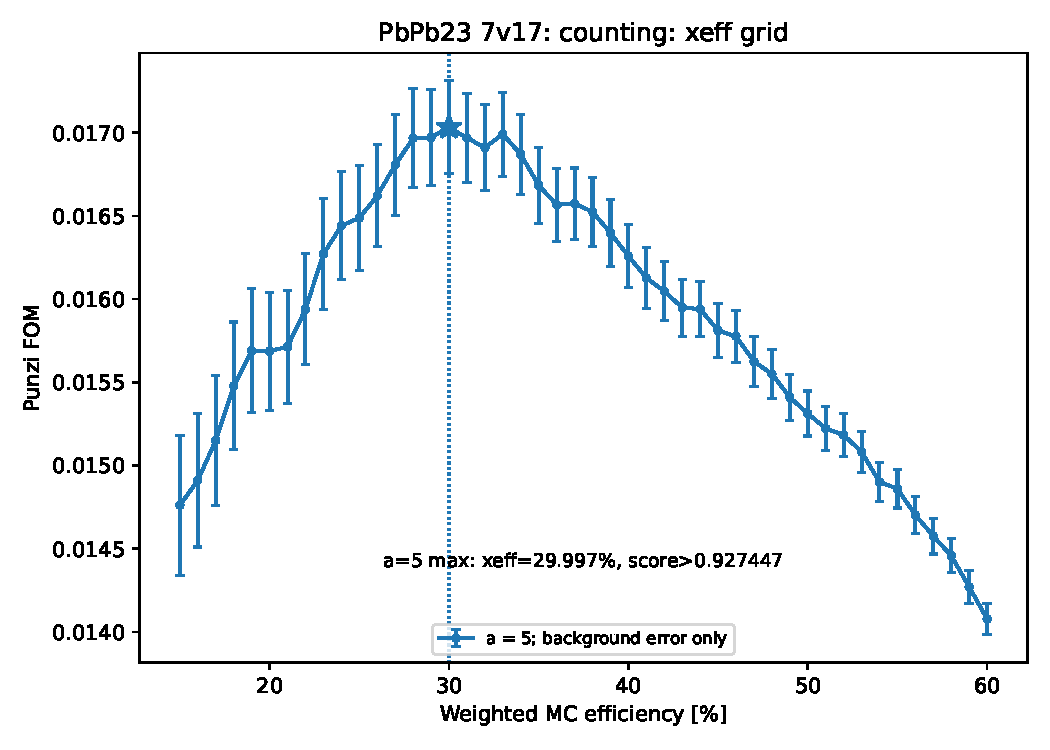
\includegraphics[width=\linewidth,height=0.56\textheight,keepaspectratio]{figures/20260920/punzi/7v17_xeff_scan_vs_xeff.pdf}
\end{columns}
\begin{itemize}\small
\item \textbf{Optimal on this grid: xeff 30\%, score $>0.927447$}; FOM $=0.017034$.
\item Points above 99\% of peak FOM: xeff 28\%--34\%; maximum is inside the grid.
\end{itemize}
\caution{Relative to 9v9: an additional track1 $\Delta R$ cut and removal of the pthat5 MC component. The shift is not attributable to variables alone.}
\end{frame}

\begin{frame}[label=p27_20260920]{7v17: fit at the Punzi-optimal cut, xeff 30\%}
\begin{columns}[c]
\column{0.65\textwidth}\centering
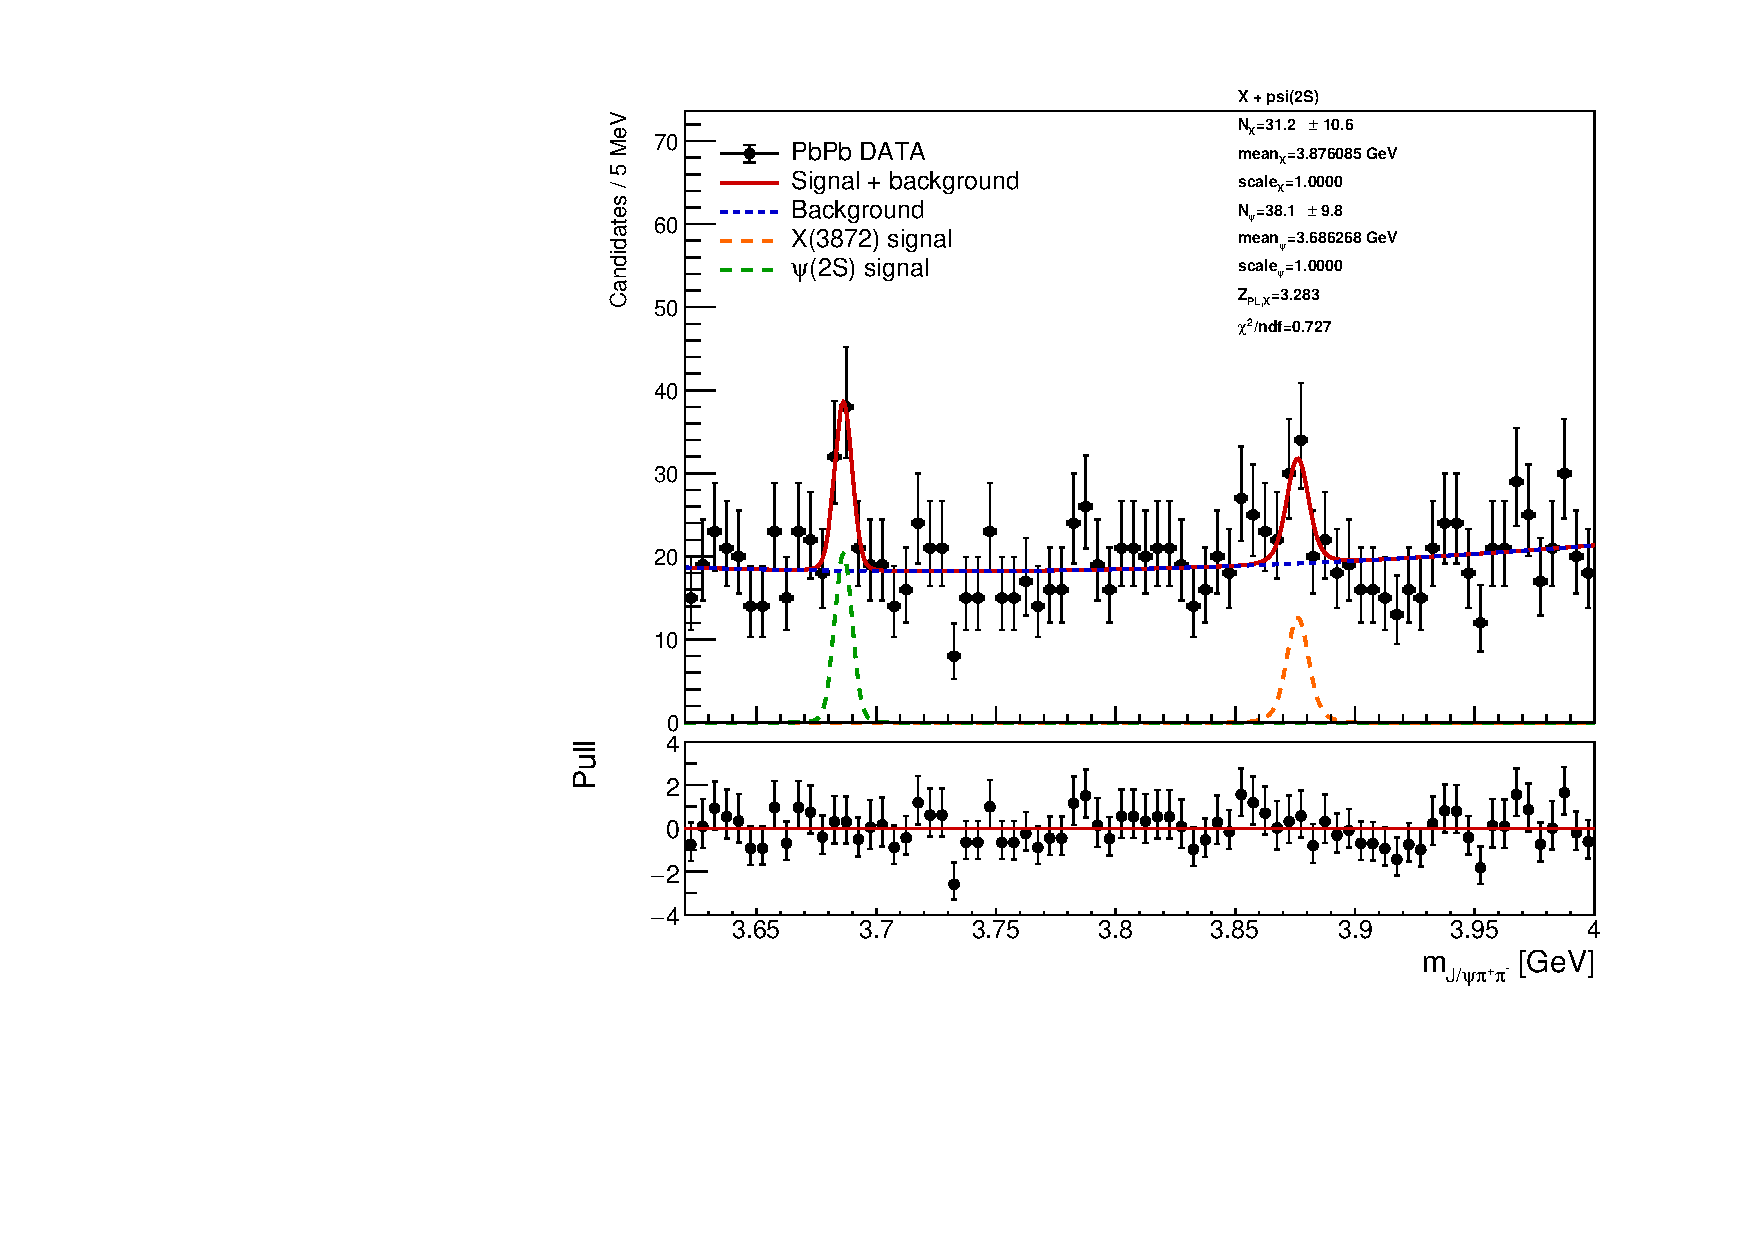
\includegraphics[width=\linewidth,height=0.65\textheight,keepaspectratio]{figures/20260920/punzi/7v17_xeff30_profile.pdf}
\column{0.33\textwidth}\small
\textbf{score $>0.927447$}\par\medskip
$N_X=31.17\pm10.59$\par
$N_{\psi(2S)}=38.15\pm9.83$\par\medskip
MC widths fixed;\par DATA means float independently; C2 background.\par\medskip
Profile $\sqrt{q_0}=3.283$\par
\end{columns}
\takeaway{Interim conclusion: use the 30\% grid optimum for the fit display; final nominal working point remains open.}
\end{frame}
